\section{Bases de datos no relacionales. NoSQL}

Las bases de datos no relacionales son un \textbf{modelo nuevo} que se ha puesto muy de moda entre desarrolladores Full Stack porque \textbf{no requiere un alto conocimiento académico de bases de datos y su curva de aprendizaje y practicidad lo hacen bastante atractivo para proyectos rápidos}.

NoSQL se compone generalmente de bases de datos, compuestas a su vez por Colecciones que poseen documentos; también hay otras tecnologías NoSQL que poseen columnas y estructuras diferentes

\subsection{Tipos de base de datos no relacionales}

No existe una clasificación universalmente aceptada en las bases de datos NoSQL. A menudo, sin embargo, suelen clasificar las bases de datos según su modelo de datos. Los cinco principales modelos de datos son: bases de datos clave-valor, documentales, orientada a grafos, orientada a columnas y orientada a objetos \cite{ref1}.

\subsubsection{Bases de datos clave-valor}

Las bases de datos clave-valor son bastante simplistas, pero tienen un modelo bastante eficiente y potente. Los datos están formados en dos partes, una cadena que representa la clave y los datos reales a los que se hace referencia como valor, creando así un par \textbf{“clave-valor”}, que es una clave única con la que se identifica cada elemento. El almacén de datos es similar a las tablas de hash donde las claves se utilizan como índices por lo que es más rápido que una base de datos relacional. Los más recientes almacenes de datos prefieren una alta escabilidad sobre la consistencia, por lo tanto, se han omitido operaciones como los joins o funciones de agregado. Algunas bases de datos de este tipo son \textit{Cassandra, Amazon DynamoDB, RIAK}.

\begin{figure}[!h]
	\centering
	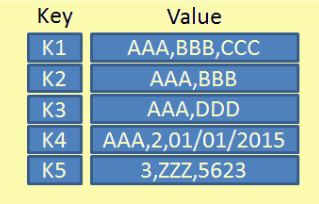
\includegraphics[scale=0.5]{images/nosql_clave-valor}
	\caption{Ejemplo de base de datos clave-valor}
	\label{fig:bd_clave-valor}
\end{figure}

\subsubsection{Bases de datos documentales}

Las bases de datos documentales almacenan sus datos en forma de documentos, generalmente
utilizando como estructura JSON (JavaScript Object Notation) o XML (Extensible Markup
Language). El almacenamiento en documentos ofrece un gran rendimiento y permite la escabilidad
horizontal. Los documentos dentro de una base de datos documental son similares a los registros
dentro de una base de datos relacional pero mucho más flexibles. En las bases de datos relacionales,
un registro dentro de la misma base de datos tendrá los mismos campos para todos los datos y los
campos que no se utilicen se mantendrán vacíos, en las bases de datos documentales cada
documento podrá tener datos similares, así como datos diferentes. Los documentos de la base de
datos utilizan una clave única que representa cada documento. Permite realizar búsquedas por
clave-valor y consultas más complejas sobre el contenido de los datos. Algunas bases de datos de
este tipo son \textit{MongoDB, CouchDB, SimpleDB \ldots}

\begin{figure}[!h]
	\centering
	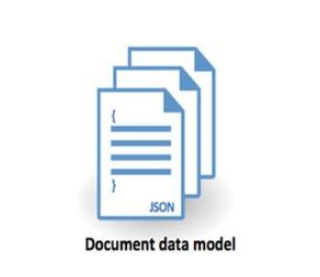
\includegraphics[scale=0.5]{images/nosql_documentos}
	\caption{Ejemplo de base de datos documental}
	\label{fig:nosql_documental}
\end{figure}

\subsubsection{Bases de datos orientadas a grafos}

Las bases de datos orientadas a grafos representan las entidades como nodos de un grafo y las relaciones como las aristas entre ellos. Utiliza una técnica llamada adyacencia libre de índice (index-free  adjacency) la cual consiste en que cada nodo tiene un puntero que apunta al nodo adyacente.  La  base  de  datos  debe  estar  totalmente  normalizada  para  poder  sacar  el  máximo rendimiento, es decir que cada tabla tendrá una sola columna y cada relación dos. De esta manera se puede adaptar el modelo de datos según las necesidades y poder recorrer millones de registros. Algunas bases de datos de este tipo son \textit{Neo4j, ArangoDB, AllegroGraph}.

\begin{figure}[!h]
	\centering
	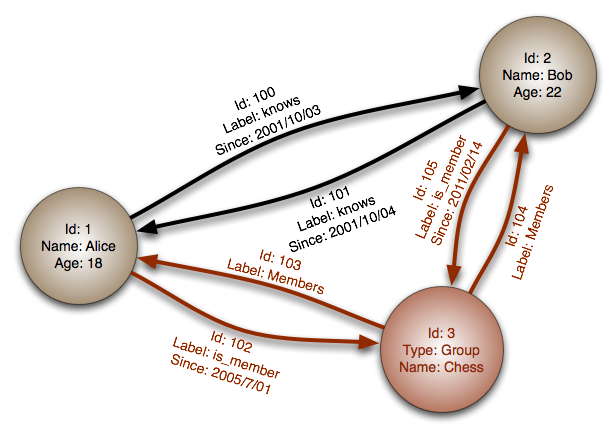
\includegraphics[scale=0.4]{images/nosql_grafos}
	\caption{Ejemplo de base de datos de grafos}
	\label{fig:nosql_grafos}
\end{figure}

\subsubsection{Bases de datos orientadas a columnas}

Son bases de datos similares a las bases de datos relacionales, aunque comparten el concepto de almacenamiento columna a columna de las bases de datos basadas en filas, los almacenes de columnas no almacenan los datos en tablas sino en arquitecturas distribuidas masivamente. En estos  almacenes  cada  clave  está  asociada  con  uno  o  más  atributos  (columnas).    Los  datos almacenados en la base de datos se basan en el orden determinado por la clasificación de la column family y se almacenan de manera contigua de tal forma que se realizan los accesos mucho más rápido. Algunas bases de datos de ese tipo son \textit{Cassandra, BigTable, HyperTable}.

\begin{figure}[!h]
	\centering
	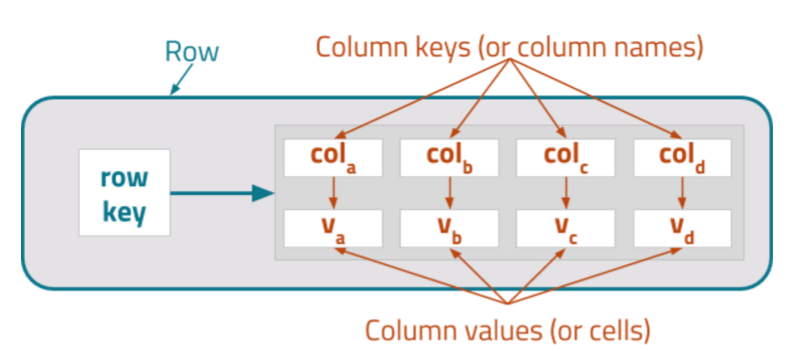
\includegraphics[scale=0.5]{images/nosql_columnas}
	\caption{Ejemplo de base de datos orientadas a columnas}
	\label{fig:nosql_columnas}
\end{figure}

\subsubsection{Bases de datos orientadas a objetos}

Son bases de datos en las cuales los datos o la información a almacenar se representan como un objeto (similar al de programación orientada a objetos). El almacén de datos ofrece todas las características  de  la  programación  orientada  a  objetos  tales  como  encapsulación  de  datos, polimorfismo y herencia. Las clases, los objetos y los atributos de clase son comparables a una tabla, una tupla y las columnas de la tupla. Cada objeto tiene un identificador que puede utilizarse para identificarlo de forma única. Las bases de datos orientadas a objetos deben utilizarse en aplicaciones que impliquen relaciones de objetos complejas o en las que cambien la estructura de objetos. Algunas bases de datos de este tipo son ObjectDB, db4o.

\begin{figure}[!h]
	\centering
	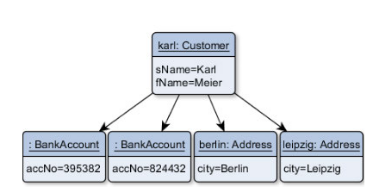
\includegraphics[scale=0.7]{images/nosql_objetos}
	\caption{Ejemplo de base de datos de objetos}
	\label{fig:nosql_objetos}
\end{figure}

\newpage

Las principales ventajas de este modelo son \cite{ref9}:

\begin{itemize}
	\item La \textbf{escalabilidad} y su carácter \textbf{descentralizado}. Soportan estructuras distribuidas.
	
	\item Suelen ser bases de datos mucho más \textbf{abiertas y flexibles}. Permiten adaptarse a necesidades de proyectos mucho más fácilmente que los modelos de Entidad Relación.
	    
	\item Se pueden hacer cambios de los esquemas sin tener que parar bases de datos.
	    
	\item \textbf{Escalabilidad horizontal}: son capaces de crecer en número de máquinas, en lugar de tener que residir en grandes máquinas.
	    
	\item Se pueden ejecutar en máquinas con pocos recursos.
	    
	\item Optimización de consultas en base de datos para grandes cantidades de datos.
\end{itemize}

Las principales inconvenientes de este modelo son \cite{ref9}:

\begin{itemize}
	\item No todas las bases de datos NoSQL contemplan la \textbf{atomicidad} de las instrucciones y la \textbf{integridad} de los datos. Soportan lo que se llama consistencia eventual.
	
	\item \textbf{Problemas de compatibilidad} entre instrucciones SQL. Las nuevas bases de datos utilizan sus propias características en el lenguaje de consulta y no son 100\% compatibles con el SQL de las bases de datos relacionales. El soporte a problemas con las queries de trabajo en una base de datos NoSQL es más complicado.
	
	\item \textbf{Falta de estandarización}. Hay muchas bases de datos NoSQL y aún no hay un estándar como sí lo hay en las bases de datos relacionales. Se presume un futuro incierto en estas bases de datos.
	
	\item \textbf{Soporte multiplataforma}. Aún quedan muchas mejoras en algunos sistemas para que soporten sistemas operativos que no sean Linux.
	
	\item Suelen tener \textbf{herramientas de administración no muy usables} o se accede por consola.
\end{itemize}

\newpage